% Anonymous venue-limited twin of ICE_paper_v2.tex. Evaluates frozen system v2.
% Official ACL style, unmodified. Canonical archival source remains separate.
\documentclass[11pt]{article}
\usepackage[review]{acl}
\usepackage{times}
\usepackage{latexsym}
\usepackage[T1]{fontenc}
\usepackage[utf8]{inputenc}
\usepackage{microtype}
\usepackage{booktabs,array,graphicx,amsmath,amssymb}
\usepackage{tikz,pgfplots}
\pgfplotsset{compat=1.18}
\usetikzlibrary{arrows.meta,positioning}
\newcolumntype{L}[1]{>{\raggedright\arraybackslash}p{#1}}
% Generated by experiments/paper/generate_analysis_tables.py; do not edit.
\newcommand{\LexicalDelta}{-0.74}
\newcommand{\LexicalCI}{[-1.14,-0.36]}
\newcommand{\FusionDelta}{+0.82}
\newcommand{\FusionCI}{[+0.39,+1.24]}
\newcommand{\FusionBareCI}{[-0.18,+0.34]}
\newcommand{\FullBareCI}{[-0.24,+0.42]}
\newcommand{\FullVectorCI}{[-0.38,+0.25]}

\title{LSREP: A Longitudinal State-Replay Protocol for Evaluating Conversational Memory, with ICE v2 as an Audited Local-First Architecture}
\author{Anonymous Authors}
\begin{document}
\maketitle
\begin{abstract}
Conversational memory changes during use, so endpoint question answering alone cannot establish how persistent state accumulates, ages, or incorporates revisions. We introduce LSREP, a longitudinal state-replay protocol with explicit lifecycle schedules, repeated probes, evolving references, and mechanism-fidelity checks. Its architectural case study is frozen ICE v2, a local-first middleware with typed stores, retrieval fusion, and dynamic context budgets. Across four private single-user datasets, 219 probes yield 1,211 checkpoint observations. Ordinary-density mean quality differences from vector-RAG are near zero; a dense workload exposes failures of the unbudgeted baseline. The audit reveals defective and unexercised mechanisms. Complementary matched LongMemEval testing shows decisive losses: ICE achieves 50.8\% versus vector's 72.8\% in the oracle and 43.0\% versus 69.5\% in full-S. Conservative abstention accompanies severe multi-session and temporal failures. Lower context use establishes a quality--cost trade-off, not superior efficiency. The disagreement shows why longitudinal evaluation, system-fidelity auditing, and public end-task testing are jointly necessary.
\end{abstract}

\section{Introduction}
A persistent memory system does more than retrieve passages. It decides what to retain, how to represent revisions, which old records to age, and how much context to supply on the next turn. These decisions change the state that later queries encounter. A correct answer at a single endpoint cannot show whether a system incorporated a revision at the appropriate time, nor whether the architecture credited for that answer actually executed.

Long-context tests reveal failures even when evidence is present in the input~\citep{liu2024lost,hsieh2024ruler}. Conversational benchmarks including LoCoMo and LongMemEval test valuable long-horizon capabilities~\citep{maharana2024locomo,wu2025longmemeval}. We add a different evaluation object: the reconstructed state trajectory of a memory system during continuing use. This is complementary to endpoint QA across supplied histories, not a replacement for it.

Our primary contribution is \textbf{LSREP}, a system-independent specification for ordered replay, declared state transitions, repeated queries, and evolving reference answers. We make its validity conditions explicit and illustrate a fact revision at two checkpoints. Its architectural contribution and case study is \textbf{ICE v2}, a local-first memory middleware with a typed persistent state, heterogeneous retrieval, rank fusion, and dynamic budgets. A retrospective fidelity audit distinguishes executed mechanisms from defective or unexercised ones.

The evaluation asks three questions. \textbf{RQ1:} How does quality and context use change under longitudinal replay? \textbf{RQ2:} Which mechanisms were live and what can be attributed to them? \textbf{RQ3:} Do the findings transfer to LongMemEval oracle and full-S conditions under a matched answerer and judge?

The answers bound the contribution. ICE v2's ordinary-density LSREP mean difference from vector-RAG is near zero. Its apparent overall advantage is largely a density-failure result against an unbudgeted baseline. On matched LongMemEval, ICE loses by 22.0--26.5 percentage points. The oracle deficit rules out distractors as the root cause. Architecture descriptions, replay scores, and public benchmark scores each omit information supplied by the other two.

\section{Related Work}
Retrieval-augmented generation supplies external evidence to an answer model~\citep{lewis2020rag,guu2020realm,izacard2021fid}. Retrieval and prompt construction are therefore part of a system's observed score. Rank fusion combines heterogeneous rankings without requiring comparable raw scores~\citep{cormack2009rrf}; it does not guarantee that adding a retrieval leg improves QA.

MemoryBank, MemGPT, and Generative Agents develop persistent or hierarchical memory and reflection~\citep{zhong2024memorybank,packer2023memgpt,park2023generative}. Mem0 includes explicit memory-update operations~\citep{chhikara2025mem0}; Zep and Hindsight organise temporally or semantically structured memory~\citep{rasmussen2025zep,latimer2025hindsight}. HippoRAG and graph-based retrieval use relations to connect evidence~\citep{gutierrez2024hipporag,edge2024graphrag}. These motivate auditing storage, retrieval, and updating separately. Their architectural mechanisms cannot be credited to ICE merely because it exposes similarly named components.

Multi-session conversation~\citep{xu2022msc}, LoCoMo, and LongMemEval expose long-term dependencies and supplied-history QA. LSREP instead requires an explicit reconstruction of state at successive checkpoints, including permitted query-induced reinforcement. Its reference may change as the supplied history changes. This specification is designed for different memory systems, but empirical portability beyond this single-user case study remains untested.

LLM judges enable scalable free-form assessment but introduce position, verbosity, and other biases~\citep{zheng2023judging,liu2023geval,wang2024unfair}. A fixed rubric and anonymised answers mitigate some risks; they do not validate labels. Our non-official LongMemEval judge permits within-study comparisons, not direct leaderboard rankings.

\section{LSREP}
\subsection{Evaluation Object and Contract}
Let $H_{\leq t}$ be the history available at checkpoint $t$, $S_t$ persistent state, $L_t$ a declared maintenance schedule, and $A_t$ allowed query side effects. A versioned system with parameters $\theta$ reconstructs
\begin{equation}
 S_t=F(S_{t-1},H_{(t-1,t]},L_t,A_{t-1};\theta).
\end{equation}
A probe $q$ has origin $o(q)$ and reference $G(q,t)$ supported only by $H_{\leq t}$. Each observation records the answer, score, actual supplied context, and observable query-induced state changes. This is a reconstructed trajectory, not exact recovery of an unlogged deployment.

An admissible implementation exposes ingestion, queries, reset or snapshots, and sufficient lifecycle control to declare maintenance and access effects. A vector index is valid: its lifecycle may simply append turns. Graphs, decay, and ICE-specific stores are not prerequisites. A chat endpoint without state control is insufficient.

\begin{figure}[t]
\fbox{\begin{minipage}{0.93\columnwidth}\small
\textbf{Algorithm 1: State replay}\par
\textbf{Input:} history, checkpoints, conditions, lifecycle/access policy, probes, reference versions.
\begin{enumerate}
\item Freeze system, models, parameters, clocks, and randomisation. Initialise declared state.
\item At each checkpoint, ingest only newly available turns in order. Complete and audit the scheduled writes and maintenance.
\item Load or construct prefix-grounded references for eligible probes, preserving their referents.
\item Query every condition. Record scope, selected context, answer, costs, component activity, and side effects. Restore snapshots when mutations are excluded.
\item Judge with a fixed rubric and missing-output policy. Aggregate paired observations while retaining probe and conversation identities.
\end{enumerate}
\textbf{Output:} a versioned observation ledger, trajectories, and scoped fidelity claims.
\end{minipage}}
\caption{LSREP specification. The historical v2 implementation does not retroactively satisfy every instrumentation requirement.}
\label{fig:protocol}
\end{figure}

\subsection{Evolving References and Validity}
A reference preserves the tracked referent, supporting evidence, answer, and prior versions. A current-truth question changes its answer when a later turn revises the fact. An explicitly historical question retains its earlier answer. Ambiguous revisions need adjudication or an uncertainty label; references must remain outside retrievable state.

\textbf{Temporal validity} excludes future evidence. \textbf{Replay validity} declares ageing, maintenance, and access events. Reconstructing a checkpoint without prior allowed reinforcement is a different trajectory. \textbf{Measurement validity} requires complete prompt accounting and inspectable missing-output and judging rules. \textbf{Mechanism validity} traces eligibility, execution, selection, and prompt inclusion; utility additionally requires a controlled contrast. \textbf{Statistical validity} states the sampling unit and target population. Deterministic schedules alone cannot guarantee identical model outputs.

\subsection{Synthetic Worked Example}
At $T_1$, an invented user states, ``The review is on Tuesday.'' The current-truth question ``When is the review?'' has reference \emph{Tuesday}. At $T_2$, new evidence says, ``Move the review to Thursday.'' The same question's reference becomes \emph{Thursday}. The historical question ``What day was originally planned?'' still has reference \emph{Tuesday}. A system repeating Tuesday at $T_2$ fails the current-truth query even though it retrieves a once-correct fact. This illustrates LSREP; it is not an additional ICE v2 experiment or private corpus excerpt.

\section{ICE v2 Architecture and Audit Contract}
\label{sec:architecture}
ICE v2 is a local-first OpenAI-compatible middleware between a client and locally served answer models. The frozen evaluation version uses FastAPI, PostgreSQL/pgvector, and Celery/Redis workers. Current ICE v3 development is independent and supplies no evidence for this paper.

\begin{figure}[t]
\centering
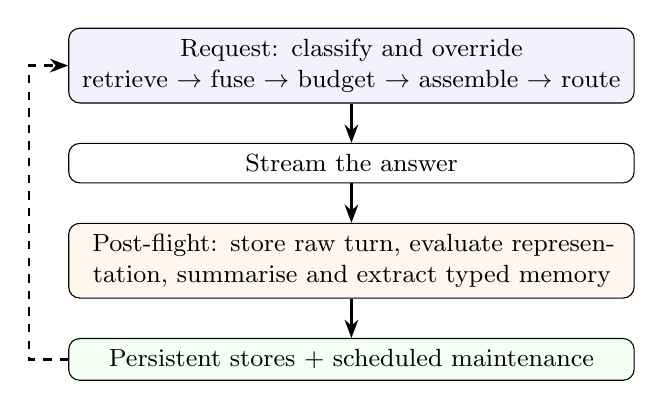
\begin{tikzpicture}[box/.style={draw,rounded corners,align=center,font=\small,text width=69mm,inner sep=4pt},arr/.style={-{Stealth},thick}]
\node[box,fill=blue!5] (pre) {Request: classify and override\\retrieve $\to$ fuse $\to$ budget $\to$ assemble $\to$ route};
\node[box,below=5mm of pre] (answer) {Stream the answer};
\node[box,below=5mm of answer,fill=orange!7] (post) {Post-flight: store raw turn, evaluate representation, summarise and extract typed memory};
\node[box,below=5mm of post,fill=green!5] (state) {Persistent stores + scheduled maintenance};
\draw[arr] (pre)--(answer);\draw[arr] (answer)--(post);\draw[arr] (post)--(state);
\draw[arr,dashed] (state.west)--++(-5mm,0)|-(pre.west);
\end{tikzpicture}
\caption{Frozen ICE v2 lifecycle. Dashed path reads evolving state on later requests. Component execution and quality benefit are separate audit questions.}
\label{fig:architecture}
\end{figure}

\textbf{Typed state.} Episodic records store turn text, summaries, embeddings, and access/decay metadata. A Codex graph keeps entities and relations with validity intervals: single-valued updates can expire earlier edges while retaining history. Procedural records represent reusable patterns; document records support external material. Memory slots and topical clusters provide structured overlays. Raw turns are stored before evaluation: ``lossless'' flags govern later representation, not whether the raw turn was stored. A validity interval denotes stored current status, not independently verified truth.

\textbf{Retrieval and assembly.} A classifier over Qwen3 embeddings provides topic, intent, and reliance labels. Conservative overrides invoke retrieval in most long-conversation turns. Six defined legs cover lexical search, decay-weighted vector similarity, graph traversal, procedures, documents, and batch summaries. The leg named BM25 actually uses PostgreSQL \texttt{ts\_rank}. Weighted reciprocal rank fusion combines candidates; sequential bonuses, foreign-session caps, deduplication, and a two-phase budget select context. Assembly includes instructions, active slots, recent turns, selected fragments, a boundary acknowledgement, and the live query. The normal leg calls are sequential, not parallel.

\textbf{Dynamic budget.} The nominal allowance is 23,000 estimated tokens, with a 1,800 reserve. Turn count, density, and classifier labels divide context between recent turns and retrieval. A growth cap gives an empty current conversation only 2,000 estimated retrieval tokens, even when other sessions hold extensive history. First-pass selection favours source-type diversity; it is not one fragment per leg. Estimates use $\lfloor1.33\times\text{words}\rfloor$, not the answerer's tokenizer. Selected episodic records are strengthened, so evaluation accesses can affect later state.

\textbf{Local operation and auditability.} Post-flight writes and scheduled decay, clustering, reflection, and consolidation maintain state. Local serving and inspectable database records are architectural properties; the cloud public diagnostic is not an all-local evaluation. Auditing must distinguish an executed error, an empty store, a constant ablation flag, and an uncertain measured effect. Non-empty output alone proves neither useful evidence nor improved answers. RQ2 applies this contract retrospectively.

\section{Evaluation Instantiation}
\subsection{LSREP Data and Conditions}
The four selected histories come from one author. They span narrative work, world-building, technical planning, and academic planning. Selection preceded scoring and sought length, complementary domains, and revisions or recurring entities. Table~\ref{tab:four} exposes every dataset and its outcome. The 1,985 turns contain about 1.98 million word-estimated tokens; 52 checkpoints repeat 219 distinct probes into 1,211 observations. Simulated ageing reaches 24, 93, 27, and 20 days in A--D. These are replay schedules, not original elapsed times.

\begin{table*}[t]
\centering\small
\resizebox{\textwidth}{!}{\begin{tabular}{@{}lrrrrrrrr@{}}\toprule
Dataset & Turns & Probes & Checkpoints & Observations & ICE score & Vector score & ICE tokens & Vector tokens\\\midrule
A: narrative & 290 & 45 & 10 & 173 & 3.63 & 3.50 & 19,434 & 24,360\\
B: world-building & 1,119 & 91 & 20 & 638 & 4.28 & 4.33 & 24,108 & 21,257\\
C: dense planning & 325 & 37 & 10 & 154 & 4.33 & 1.23 & 19,953 & 88,061\\
D: academic planning & 251 & 46 & 12 & 246 & 4.63 & 4.57 & 20,103 & 18,076\\\bottomrule
\end{tabular}}
\caption{ICE v2 LSREP coverage and generalist-arm results. Scores are the historical 1--5 rubric; tokens estimate the complete supplied prompt. C is the density stress case. Observations repeat probes and are not independent tasks.}
\label{tab:four}
\end{table*}

Each conversation is replayed chronologically with state preserved between checkpoints. Scheduled ageing and maintenance run between checkpoints. Prefix-based probes sample early, recent, and intermediate history and are combined with inherited hand-written probes. Origin references are regenerated with evidence provenance, temporally anchored, and propagated forward when later evidence changes the answer. Every eligible probe is asked again at subsequent checkpoints.

Four conditions cross full ICE versus top-30 vector-RAG with a generalist versus expert routing. Both use the same stored embeddings. The generalist is \texttt{gemma4:26b-a4b-it-q4\_K\_M}; the independent judge is \texttt{gemma-4-12B-AWQ}, served on SGLang at a 150,000-token context and requested temperature 0.0. Generalist-arm comparisons are primary here. ICE includes its assembler and budget; vector uses top-30 similarity without decay, fusion, or a token budget. This compares complete configurations, not retrieval algorithms isolated under equal prompts.

Scoring uses a temporal-aware 1--5 rubric and separate anonymised four-condition rankings. The aggregation replaces scores/rankings with 72 manual records where supplied. The corpus author also audited hallucination labels; this is not independent human validation. Missing-score fallback is explicit score, failed answer assigned 1, sibling routing score, rounded record mean, then 3. The final two fallbacks are unused. Appendix~\ref{app:sensitivity} reports source and complete-case sensitivity.

\subsection{Matched LongMemEval Diagnostic}
We evaluate all 500 oracle and full-S questions~\citep{wu2025longmemeval}. The corrected session adapter wipes state per question, ingests each supplied session into a distinct auto-scoped conversation, and asks from a fresh empty conversation. Oracle supplies evidence sessions; full-S adds the remaining histories. Vector-RAG reads the same stored vectors but selects top 30 without a token cap, decay, or fusion. It is a strong high-context baseline, not a budget-matched arm.

Both answer arms use \texttt{gpt-5.6-luna} through OpenCode Go's Responses endpoint with a 4,096-output-token cap. Temperature control was unsupported. ICE construction uses local \texttt{qwen3:4b-instruct-bg}. Muse Spark 1.3 Contributor judges both arms with the official task-specific prompts and yes/no rule, using a 4,096-token cap. Muse is not LongMemEval's official GPT-4o judge; comparisons are internal to this stack.

The adapter calls frozen v2 classification, budget setting, retrieval, and assembly. Run-enablement changes restore the shared Ollama background route and move the unchanged 384-dimensional embedder to CUDA; recorded CPU--CUDA cosine agreement is 0.99986. No v3 repair is included. The adapter omits the HTTP wrapper's faulty secondary word check, which counts instructions and question but not all supplied context. The result measures the documented adapter path, not the full HTTP lifecycle.

\subsection{Analysis Units}
Historical LSREP intervals bootstrap probe--checkpoint records. Our sensitivity instead resamples each distinct probe with its entire observed trajectory, preserving the paired arms and the observation-weighted estimand. We use 20,000 percentile resamples, seed 20260911. This captures repeated-probe dependence, not generalisation across users. Paired win/tie/loss counts supplement means without assuming equal spacing between rubric levels~\citep{nistSignTest}. Score-per-fragment and score-per-token ratios remain archival descriptors, not validated quality measures.

LongMemEval uses paired question resampling, preserving all four arm--phase outcomes for degradation comparisons. Missing judgements are excluded from paired estimates and bounded over all questions. Category intervals are exploratory and unadjusted. All uncertainty conditions on recorded generations and labels; it excludes model rerun and judge-error uncertainty.

\section{Results}
\subsection{RQ1: Longitudinal Behaviour}
On A, B, and D, ICE v2 selects 32\% fewer fragments but uses 6.6\% more estimated prompt tokens. The paired mean-score difference is $+0.002$, with historical record interval $[-0.07,+0.07]$ and wider probe-cluster interval $[-0.148,+0.158]$. This is no detected mean difference, not equivalence. Ordinary-density paired ordering gives 216 ICE-higher, 215 vector-higher, and 626 tied observations: net superiority $+0.1$ percentage points, cluster interval $[-7.6,+8.0]$.

\begin{figure}[t]
\centering
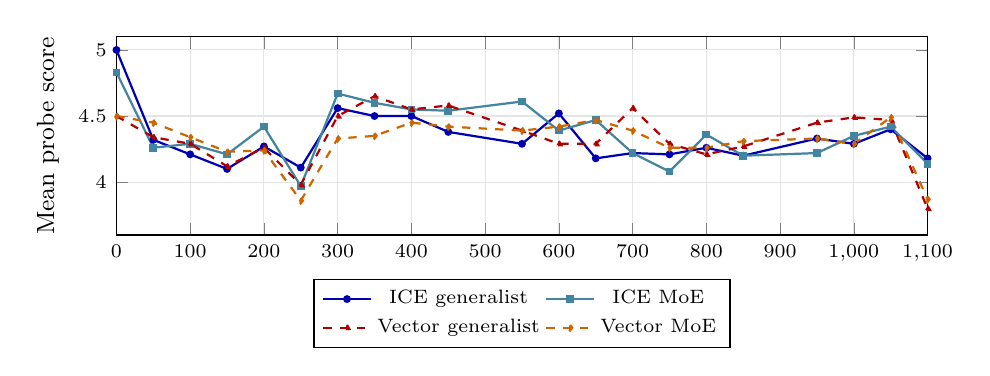
\begin{tikzpicture}
\begin{axis}[
    width=0.98\columnwidth, height=4.1cm,
    xlabel={\small Turn-index bin}, ylabel={\small Mean probe score},
    ylabel near ticks,
    xmin=0, xmax=1100, ymin=3.6, ymax=5.1,
    tick label style={font=\scriptsize},
    legend style={font=\scriptsize, at={(0.5,-0.22)}, anchor=north, legend columns=2},
    grid=major, grid style={gray!20},
]
\addplot[blue!70!black, thick, mark=*, mark size=1pt] coordinates
 {(0,5) (50,4.32) (100,4.21) (150,4.1) (200,4.27) (250,4.11) (300,4.56) (350,4.5) (400,4.5) (450,4.38) (550,4.29) (600,4.52) (650,4.18) (700,4.22) (750,4.21) (800,4.26) (850,4.2) (950,4.33) (1000,4.29) (1050,4.4) (1100,4.18)};
\addplot[cyan!60!black, thick, mark=square*, mark size=1pt] coordinates
 {(0,4.83) (50,4.26) (100,4.29) (150,4.21) (200,4.42) (250,3.97) (300,4.67) (350,4.6) (400,4.55) (450,4.54) (550,4.61) (600,4.39) (650,4.47) (700,4.22) (750,4.08) (800,4.36) (850,4.2) (950,4.22) (1000,4.35) (1050,4.42) (1100,4.14)};
\addplot[red!70!black, thick, dashed, mark=triangle*, mark size=1pt] coordinates
 {(0,4.5) (50,4.34) (100,4.29) (150,4.12) (200,4.26) (250,3.98) (300,4.5) (350,4.65) (400,4.55) (450,4.58) (550,4.39) (600,4.29) (650,4.29) (700,4.56) (750,4.29) (800,4.21) (850,4.27) (950,4.45) (1000,4.49) (1050,4.47) (1100,3.8)};
\addplot[orange!80!black, thick, dashed, mark=diamond*, mark size=1pt] coordinates
 {(0,4.5) (50,4.45) (100,4.34) (150,4.23) (200,4.24) (250,3.86) (300,4.33) (350,4.35) (400,4.45) (450,4.42) (550,4.39) (600,4.42) (650,4.47) (700,4.39) (750,4.26) (800,4.26) (850,4.31) (950,4.33) (1000,4.29) (1050,4.49) (1100,3.87)};
\legend{ICE generalist, ICE MoE, Vector generalist, Vector MoE}
\end{axis}
\end{tikzpicture}
\caption{ICE v2 LSREP mean score by turn-index bin, ordinary-density data. Query mix changes across bins; the final bin contains Dataset B only. Its separation is descriptive, not a controlled forgetting or retrieval-reach effect.}
\label{fig:longitudinal}
\end{figure}

Figure~\ref{fig:longitudinal} shows that all four conditions track closely through most turn-index bins. The final, Dataset-B-only bin separates ICE generalist (4.18) from vector (3.80), but this is a descriptive endpoint, not evidence of a general long-horizon advantage.

Removing manual replacements shifts the ordinary-density mean difference to $-0.020$ ($[-0.169,+0.136]$). The near-zero conclusion is therefore not dependent on retaining those replacements. Query mix and state both vary with checkpoint: token differences do not improve monotonically. For example, D shifts from 2,309 fewer estimated ICE tokens in the first quartile to 4,994 more in the last. Such position contrasts are descriptive, not budget interventions or forgetting estimates.

Dataset C changes the aggregate result. Its vector mean is 1.23 against ICE's 4.33, with 94.2\% versus 3.9\% score-1 observations. Across all data, the paired mean difference is $+0.396$ ($[+0.192,+0.618]$); on C alone it is $+3.097$ ($[+2.721,+3.470]$). This demonstrates resilience of the full ICE configuration relative to this unbudgeted baseline under extreme density, without isolating the budget's causal contribution.

Missing-score handling matters here. Vector generalist has 130 failed-answer assignments to 1 and two sibling-routing substitutions; ICE has 1,211 explicit scores. Keeping only pairs with explicit scores reduces the all-data difference to $+0.046$ ($[-0.101,+0.199]$, $n=1,079$). That selected subset drops most density failures and cannot replace the operational reliability comparison. Both views are necessary.

\subsection{RQ2: Mechanism Fidelity}
A cumulative buildup on 67 Dataset-B probes uses Qwen3-14B-AWQ answers and the same independent Gemma judge. Scores are paired within probe; absolute scores are not comparable with the 26B LSREP run. Adding an unfused lexical leg lowers mean score by $\LexicalDelta$ ($\LexicalCI$); adding RRF then recovers $\FusionDelta$ ($\FusionCI$). These are the only adjacent steps whose 95\% intervals exclude zero. Fusion corrects damage in this buildup; fusion versus bare vector spans zero. It is not a general guarantee that more retrieval legs help.

The audit explains why other small deltas cannot be celebrated. Procedural retrieval raises a pgvector operator error from an untyped embedding bind and returns empty. The document leg shares the defect and has no ingested documents. Batch summaries have no eligible content. HyDE is disabled in the mature run and constant rather than isolated across its nominal ablation toggle. Graph output accounts for 3.3\% of fragments, but a traversal is concatenated into one fragment; fragment share does not identify token share or graph utility. Cross-conversation caps are rarely engaged by single-conversation LSREP.

Vector and lexical retrieval, fusion, budget selection, and reinforcement execute, but execution is not individual causal attribution. Routing changes ordinary-density scores by only $+0.03$ for ICE and $-0.02$ for vector; this is a small observed difference, not proven equivalence. The audit bounds what the architecture can claim and identifies mechanisms needing dedicated evidence-level controls.

\subsection{RQ3: External Transfer}
\begin{table*}[t]
\centering\small
\begin{tabular}{@{}lrrrr@{}}\toprule
 & Oracle ICE & Oracle vector & Full-S ICE & Full-S vector\\\midrule
Abstention ($n=30$) & 83.3 & 60.0 & 83.3 & 63.3\\
Knowledge update ($n=72$) & 58.3 & 73.6 & 51.4 & 69.4\\
Multi-session ($n=121$) & 29.8 & 86.0 & 21.5 & 74.4\\
Single-session assistant ($n=56$) & 91.1 & 94.6 & 75.0 & 94.6\\
Single-session preference ($n=30$) & 70.0 & 70.0 & 43.3 & 51.7$^*$\\
Single-session user ($n=64$) & 78.1 & 95.3 & 71.9 & 93.8\\
Temporal reasoning ($n=127$) & 22.8 & 42.5 & 20.5 & 47.2\\\midrule
Overall & 50.8 & 72.8 & 43.0 & 69.5$^*$\\
Paired ICE$-$vector, points (95\% CI) & \multicolumn{2}{c}{$-22.0\;[-26.6,-17.4]$} & \multicolumn{2}{c}{$-26.5\;[-31.3,-21.8]$}\\\bottomrule
\end{tabular}
\caption{Matched LongMemEval correctness (\%). Frozen ICE v2 and pure vector-RAG share answerer and judge. $^*$One missing full-S vector judgement: preference $n=29$, overall $n=499$. All-500 bounds are ICE 43.0\% and vector 69.4--69.6\%; the ordering is robust.}
\label{tab:lme}
\end{table*}
ICE v2 loses decisively overall in both phases (Table~\ref{tab:lme}). The 22-point oracle deficit already occurs with evidence-only histories: distractors cannot be the root cause. On full-S, multi-session correctness is 21.5\% versus 74.4\%; temporal correctness is 20.5\% versus 47.2\%. These are substantial failures of aggregation and temporal composition under this adapter and stack.

Abstention is a descriptive exception: ICE answers 25/30 correctly versus vector's 19/30 in full-S. Paired cells contain seven ICE-only successes, one vector-only, 18 both-correct, and four both-wrong. The bootstrap difference is $+20.0$ points ($[+3.3,+36.7]$), but the exact two-sided McNemar test gives $p=0.0703$. With only eight discordant pairs and unadjusted category analyses, we retain the descriptive interpretation rather than a strong confirmatory advantage.

From oracle to full-S, ICE has 68 correct-to-wrong and 29 wrong-to-correct transitions over 500 questions: a 7.8-point loss. Vector has 44 and 28 over 499 complete phase pairs: a 3.2-point paired loss. On the common 499 questions, the extra ICE degradation is 4.4 points ($[-0.2,+9.2]$); its interval includes zero. The displayed marginal gaps and paired phase contrast use different denominators.

\begin{table}[t]
\centering\small
\begin{tabular}{@{}llrr@{}}\toprule
Phase & Arm & Fragments & Input tokens\\\midrule
Oracle & ICE & 3 [3,4] & 2,006 [1,758,2,118]\\
 & Vector & 11.5 [6,12] & 5,529 [3,370,6,732]\\
Full-S & ICE & 5 [4,6] & 2,222 [2,168,2,289]\\
 & Vector & 30 [30,30] & 11,718 [10,437,12,923]\\\bottomrule
\end{tabular}
\caption{Median [quartiles] selected/injected fragments and provider input tokens. Both are observed quantities, not configured caps or pre-selection candidates. All 2,000 answers have usage metadata.}
\label{tab:cost}
\end{table}

\textbf{Quality and cost.} ICE supplies less context (Table~\ref{tab:cost}) while producing substantially less accurate answers. Full-S correct and incorrect ICE answers have almost identical median input counts, 2,224 versus 2,219; vector's are 11,650 versus 11,855. Vector still fails on 31/121 multi-session questions despite supplying 30 fragments. These observational strata do not identify the cause of errors or accuracy at matched budgets.

Median generation-only times are 2.8/2.0 seconds for oracle ICE/vector and 3.1/2.6 for full-S. No answer is empty or incomplete; one vector judgement is missing. Retrieval-only tokens, candidate counts, retrieval latency, and arm-specific construction costs were not retained at the required granularity. Context economy is established, superior efficiency is not: that requires a declared quality constraint or an accuracy--token frontier.

\section{Implications and Conclusion}
LSREP and LongMemEval expose complementary regimes. The former evaluates evolving memory within continuing use; the latter tests endpoint QA across supplied histories from a fresh session. ICE v2's replay behaviour did not transfer to strong public-benchmark performance. The fidelity audit further prevents attributing either result to mechanisms that failed or never ran.

An observed benchmark score belongs to the whole stack: memory architecture, answerer, judge, prompt, budget, and dataset. Future work should hold memory systems fixed while varying answerers and crossing judge families to test ranking stability. We have not shown family-related judging bias. Numerically overlapping published scores do not establish a ranking under mismatched stacks (Appendix~\ref{app:context}). The value of complexity must be measured against strong simple baselines under matched conditions, including budget sweeps and capability-specific outcomes.

LSREP contributes a concrete evaluation contract; ICE v2 contributes an inspectable architecture and a bounded case study. Together, replay, execution auditing, and public QA make both apparent success and decisive failure more informative than either aggregate alone.

\section*{Limitations}
The private histories come from one author, and the protocol was developed alongside ICE. The 1,211 observations repeat 219 probes; cluster intervals still condition on four conversations and cannot support population claims. Manual labels share the corpus author. Model-assisted references can omit evidence or preserve authoring errors. Negative results do not prove an unbiased evaluation instrument. Independent systems, users, and public trajectories are needed.

Replay is not deployment: evaluation probes reinforce selected memories, and ordinary conversational accesses are not fully reconstructed. Conditions sharing state can affect later observations; future implementations need isolated trajectories when mutations differ. Prefix-based reference construction and temporal anchoring reduce, but do not eliminate, leakage and reference drift. Frozen v2 descriptions must not be read as current v3 behaviour.

The complete configurations differ in prompts and budgets, so their contrast does not isolate the memory architecture. The ablation uses one conversation and a smaller answer model; defective and constant paths limit attribution. Mean rubric scores assume numerical spacing, so ordinal and scoring-source sensitivities are included. Complete-case selection removes many failed answers and changes the target workload.

The public diagnostic uses a non-official Muse judge. Its three-case discrimination check and earlier 15-item calibration (73\% agreement in a different setting) are not a broad LongMemEval validation. Answerer selection used a small sample from the same benchmark. Bootstrap intervals exclude judge error, rerun variation, and selection uncertainty; category tests are exploratory. The 30-question abstention group is especially uncertain.

Provider tokens are observed, but prompt estimates in LSREP are word-based. Generation latency omits retrieval, ingestion, and retries. No matched-budget curve or end-to-end cost study establishes superior efficiency. The cloud public experiment is distinct from the architecture's local deployment capability.

\section*{Ethical Considerations}
Private conversations and probe text are not released, and this paper includes no verbatim private example. Exact private LSREP results are therefore not independently reproducible. Aggregate reports and analysis methods permit inspection without disclosing personal text; public benchmark data must be obtained from its original release. Raw answers, judgements, databases, logs, credentials, and personal planning notes are excluded from the public artifact scope. Anonymous review material must preserve the same boundary. No system was deployed to make consequential decisions for other users in this evaluation.

\section*{Declaration on Generative AI}
Generative AI tools, including Codex, assisted manuscript drafting and revision, literature discovery, analytical suggestions, and development of analysis scripts. Their use included the protocol presentation, discussion of results, and sensitivity-analysis implementation. Claims were checked against cited sources and frozen experiment records, and numerical analyses were recomputed with executable scripts and arithmetic controls. Model-assisted probe generation, reference construction, answer generation, and judging are described in the evaluation methods. Responsibility for the manuscript, interpretation, and final approval rests with the human author.

\bibliography{ICE_references}
\appendix
\section{Scoring Sensitivity and Reproducibility}
\label{app:sensitivity}
The archived LSREP analysis resamples 10,000 probe--checkpoint records. The added analyses use 20,000 whole-probe cluster resamples with seed 20260911 and retain the observation-weighted mean. Distinct probes are identified within conversation. Both arms remain together. Scores exactly reproduce the archived manual merge and fallback chain before sensitivity policies are applied.

\begin{table*}[t]
\centering\small
\begin{tabular}{llrrr}
\toprule
Scoring & Regime & $n$ & $\Delta$ & Probe-cluster 95\% CI \\
\midrule
Merged, archived & All & 1,211 & $+0.396$ & $[+0.192,+0.618]$ \\
Merged, archived & Ordinary & 1,057 & $+0.002$ & $[-0.148,+0.158]$ \\
Merged, archived & Density & 154 & $+3.097$ & $[+2.721,+3.470]$ \\
Automated, archived & All & 1,211 & $+0.363$ & $[+0.162,+0.582]$ \\
Automated, archived & Ordinary & 1,057 & $-0.020$ & $[-0.169,+0.136]$ \\
Automated, archived & Density & 154 & $+2.994$ & $[+2.606,+3.359]$ \\
Merged, complete & All & 1,079 & $+0.046$ & $[-0.101,+0.199]$ \\
Merged, complete & Ordinary & 1,055 & $+0.001$ & $[-0.148,+0.157]$ \\
Merged, complete & Density & 24 & $+2.042$ & $[+1.077,+3.294]$ \\
Automated, complete & All & 1,067 & $-0.021$ & $[-0.168,+0.128]$ \\
Automated, complete & Ordinary & 1,054 & $-0.022$ & $[-0.170,+0.131]$ \\
Automated, complete & Density & 13 & $+0.077$ & $[-0.714,+0.714]$ \\
\bottomrule
\end{tabular}

\caption{Scoring-source and complete-case sensitivity, ICE v2 minus vector generalist. Cluster intervals condition on the same private histories.}
\end{table*}

Without manual replacements, vector generalist has 1,067 explicit labels, 141 failed-answer assignments, and three sibling substitutions; with replacements, 1,079, 130, and two. ICE generalist has 1,211 explicit scores in either policy. Vector-MoE has 34 failed-answer assignments; ICE-MoE one sibling substitution. Neither the rounded-mean nor default-3 fallback is used. The automated-only complete-case density subset contains just 13 of 154 observations. It is selection-sensitive and does not estimate reliability on the original workload.

Paired ordinal net superiority is the proportion of ICE-higher scores minus vector-higher scores, with ties contributing zero. Whole-probe bootstrap uncertainty replaces an independent-observation sign test. In all merged data, counts are 355 ICE-higher, 220 vector-higher, 636 tied: net $+11.1$ points ($[+3.2,+19.5]$). Density-only net is $+87.0$ ($[+77.5,+95.3]$); ordinary-density results are in the main text. These summaries use ordering without treating score ratios as measures of utility.

The analyses make no model or database calls and export aggregate tables only. Paired LongMemEval statistics preserve question identity across arms and phases. Source hashes identify the locally retained evidence without exporting question identifiers. The ablation report reuses each contrast across step, cumulative, and headline views, avoiding Monte Carlo drift from repeated resampling of the same contrast.

\section{Additional ICE v2 Fidelity Details}
The graph models property relations, accumulating multi-valued relations, and superseding single-valued relations. Ended validity intervals retain history. Extraction and retrieval quality remain unconfirmed by structural presence alone. The trained NER checkpoint was loaded, but no task-specific recall estimate is established here.

Access-weighted decay, topical clustering, reflection, and summarisation are architectural maintenance paths. Memory slots carry explicitly managed persistent context. Retrieval source-type diversity groups lexical and vector results together as episodic; it is not diversity across all six legs. A foreign conversation can contribute at most three selected fragments, while the active conversation is uncapped by that rule. The fresh empty LongMemEval question scope therefore differs materially from continuing-use LSREP.

The API wrapper's final word-budget check omits retrieved and recent messages, so it is not a full prompt-size guarantee. Both evaluated adapters call selection/assembly directly rather than this wrapper. The v2 retrieval budget is live, but the density full-system contrast cannot establish its independent effect. Its cumulative buildup step is $-0.08$ with interval $[-0.36,+0.18]$. Cluster restriction and session diversity also have intervals spanning zero. Document retrieval's operator defect and absent content are separate limitations; neither is evidence that external documents would not help a repaired system.

The earlier flattened-session LongMemEval adapter was invalidated after a string/UUID mismatch incorrectly triggered foreign-session capping. Only the corrected session-preserving adapter enters the main results. A prior local-Gemma oracle obtained ICE 264/478 and vector 388/484 judged-correct answers, with missing-label bounds 52.8--57.2\% and 77.6--80.8\%. It stopped before full-S and is historical evidence only; the later matched cloud study completed both phases. No scores from that older run enter the main matched tables.

\begin{table*}[t]
\centering\small
\begin{tabular}{@{}llrrrrrr@{}}
\toprule
Phase & Category & Both correct & ICE only & Vector only & Both wrong & $n$ & $\Delta$ [95\% CI], pp\\\midrule
Oracle & Abstention & 17 & 8 & 1 & 4 & 30 & $+23.3 [+6.7,+40.0]$ \\
Oracle & Knowledge update & 37 & 5 & 16 & 14 & 72 & $-15.3 [-27.8,-2.8]$ \\
Oracle & Multi-session & 36 & 0 & 68 & 17 & 121 & $-56.2 [-65.3,-47.1]$ \\
Oracle & Session assistant & 49 & 2 & 4 & 1 & 56 & $-3.6 [-12.5,+5.4]$ \\
Oracle & Session preference & 18 & 3 & 3 & 6 & 30 & $+0.0 [-16.7,+16.7]$ \\
Oracle & Session user & 49 & 1 & 12 & 2 & 64 & $-17.2 [-28.1,-7.8]$ \\
Oracle & Temporal & 22 & 7 & 32 & 66 & 127 & $-19.7 [-28.3,-10.2]$ \\
Full-S & Abstention & 18 & 7 & 1 & 4 & 30 & $+20.0 [+3.3,+36.7]$ \\
Full-S & Knowledge update & 31 & 6 & 19 & 16 & 72 & $-18.1 [-30.6,-5.6]$ \\
Full-S & Multi-session & 24 & 2 & 66 & 29 & 121 & $-52.9 [-62.8,-43.0]$ \\
Full-S & Session assistant & 41 & 1 & 12 & 2 & 56 & $-19.6 [-32.1,-8.9]$ \\
Full-S & Session preference & 9 & 4 & 6 & 10 & 29 & $-6.9 [-27.6,+13.8]$ \\
Full-S & Session user & 46 & 0 & 14 & 4 & 64 & $-21.9 [-32.8,-12.5]$ \\
Full-S & Temporal & 22 & 4 & 38 & 63 & 127 & $-26.8 [-35.4,-18.1]$ \\
\bottomrule\end{tabular}
\caption{Paired cells and exploratory question-bootstrap uncertainty. Positive differences favour ICE v2. Full-S preference excludes the missing vector judgement. Intervals are unadjusted and conditional on recorded labels.}
\end{table*}
\section{Published-System Context}
\label{app:context}
Published LongMemEval-S numbers are contextual, not comparable rankings. Zep reports 63.8\% with GPT-4o-mini and 71.2\% with GPT-4o, using GPT-4o judging and task-specific official judgement prompts; its mean context is about 1.6K tokens, not a declared common cap~\citep{rasmussen2025zep}. Its retrieval and answer prompt differ from ours.

Hindsight v1 reports 83.6\% using GPT-OSS-20B and 91.4\% using Gemini-3 Pro, with GPT-OSS-120B judging and paper-specific templates. The Gemini condition uses OSS-120B memory construction; v1 does not supply a usable retrieval-budget value~\citep{latimer2025hindsight}. These differences in answerer, judge, prompts, retrieval, and memory protocol prevent direct ranking against ICE or vector. A matched rerun, or appropriately controlled official-judge re-evaluation, is required for a direct comparison.
\section{Paired LongMemEval Category Ledger}

The oracle abstention contrast has eight ICE-only and one vector-only success; the full-S contrast has seven and one. Small discordant samples explain why asymptotic or bootstrap interval heuristics should not replace a cautious descriptive interpretation. No category analysis incorporates judge misclassification.

Oracle-to-full ICE degradation is 7.8 points with interval $[4.0,11.6]$ over 500 questions. Vector degradation is 3.2 points with interval $[-0.2,6.4]$ over 499. The extra ICE degradation uses the common 499-question set, so its 4.4-point estimate is not the simple subtraction of rounded marginal accuracies.

Generation time median [quartiles], in seconds, is 2.8 [2.2,3.4] for oracle ICE, 2.0 [1.6,2.8] for oracle vector, 3.1 [2.5,3.8] for full-S ICE, and 2.6 [2.1,3.5] for full-S vector. All answer records are complete and nonempty; this does not measure transient retries.
\end{document}
